\documentclass{standalone}
\usepackage{tikz}
\usepackage{newtxmath}

\begin{document}

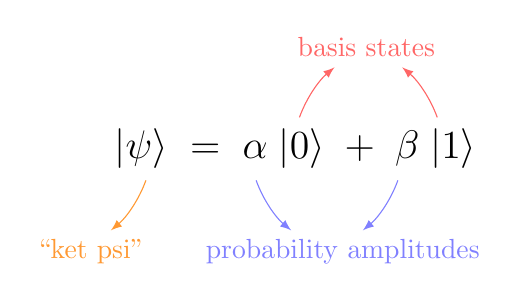
\begin{tikzpicture}
    \node[] at (0,0) {\Large $|\psi\rangle \; = \; \alpha \; |0\rangle \; + \; \beta \; |1\rangle$};
    
    \draw[-latex,red!60] (0.05,0.4) arc[start angle=160, end angle=130, radius=1.5];
    \draw[-latex,red!60] (1.8,0.4) arc[start angle=20, end angle=50, radius=1.5];
    \node[red!60] at (0.9,1.3) {basis states};

    \draw[-latex,blue!50] (-0.5,-0.4) arc[start angle=200, end angle=230, radius=1.5];
    \draw[-latex,blue!50] (1.3,-0.4) arc[start angle=340, end angle=310, radius=1.5];
    \node[blue!50] at (0.6,-1.3) {probability amplitudes};

    \draw[-latex,orange!80] (-1.9,-0.4) arc[start angle=340, end angle=310, radius=1.5];
    \node[orange!80] at (-2.6,-1.3) {``ket psi''};
\end{tikzpicture}

\end{document}